\label{sec:workorder}

На рисунке~\ref{fig:main_page} представлена главная страница системы голосовой аутентификации. Справа расположен логотип системы, под которым отражается статус пользователя (авторизован или нет). В центральной части страницы находится ссылка для перехода на страницу аутентификации и форма ввода имени учетной записи.
В нижней части представлена <<Навигация>>, которая состоит из ссылки на регистрацию в системе и ссылки для перехода на главную страницу защищаемого интернет-ресурса. Если пользователь не авторизован на интернет-ресурсе, то в списке <<Навигация>> присутствует ссылка на страницу с формой ввода имени учетной записи и пароля. Если пользователь авторизован, то вместо ссылки на страницу с формой ввода имени учетной записи и пароля присутствует ссылка <<Выход>>.

\begin{figure}[hbt!]
\center{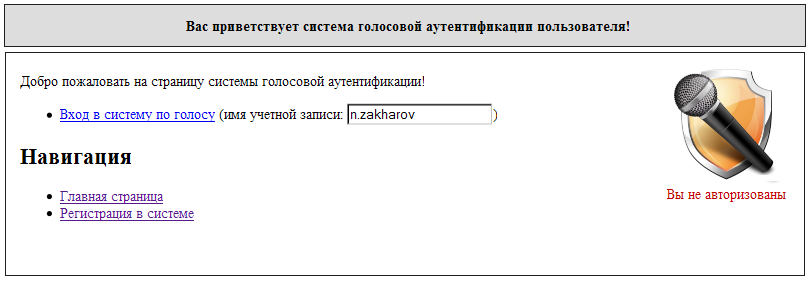
\includegraphics[width=\textwidth]{static_include/main_page.png}}
\caption{Главная страница системы голосовой аутентификации}
\label{fig:main_page}
\end{figure}

При выборе пункта <<Регистрация в системе>> пользователь автоматически переходит на страницу, которая содержит список требований, удовлетворение которых необходимо для регистрации в системе. Если пользователь авторизован на интернет-ресурсе, на странице присутствует ссылка для перехода к созданию персональной голосовой модели (рисунок~\ref{fig:enrollment_initial_authentificated}). Если пользователь не авторизован, на странице отображается сообщение о необходимости авторизации (рисунок~\ref{fig:enrollment_initial_anonymous}).

\begin{figure}[hbt!]
\center{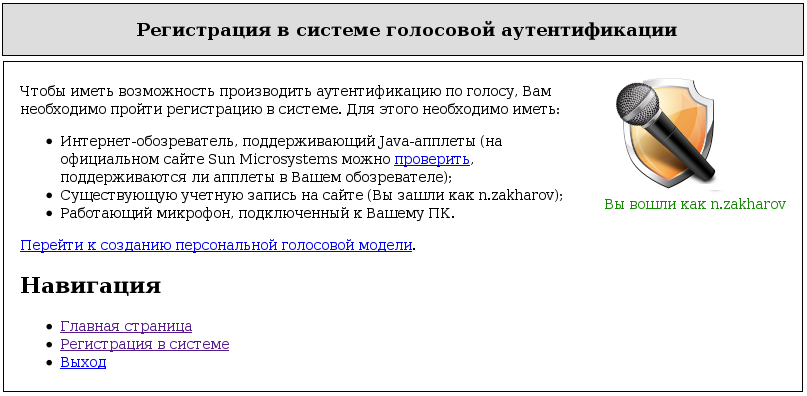
\includegraphics[width=\textwidth]{static_include/enrollment_initial_authentificated.png}}
\caption{Информация о регистрации (пользователь авторизован)}
\label{fig:enrollment_initial_authentificated}
\end{figure}

\begin{figure}[hbt!]
\center{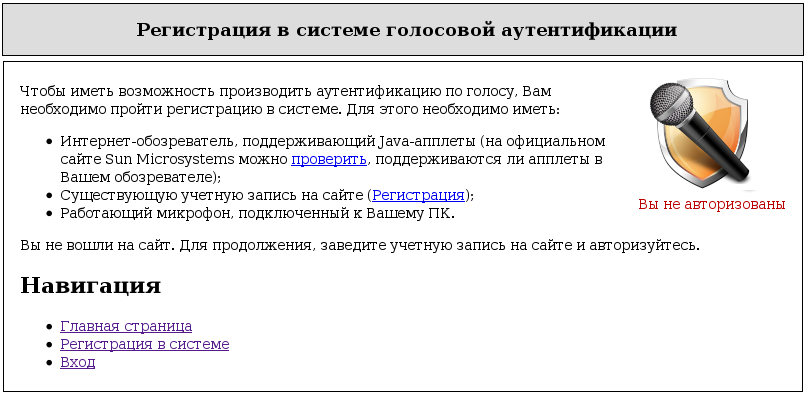
\includegraphics[width=\textwidth]{static_include/enrollment_initial_anonymous.png}}
\caption{Информация о регистрации (пользователь не авторизован)}
\label{fig:enrollment_initial_anonymous}
\end{figure}

\subsubsection{Создание индивидуальной голосовой модели}
\label{sec:manual:enrollment}

В случае выбора ссылки <<Перейти к созданию индивидуальной голосовой модели>>,
производится переход к странице с формой, которая представлена на
рисунке~\ref{fig:enrollment_created}. В центральной части формы находится
краткая инструкция по записи образца ключевой фразы. В нижней части находится
кнопка <<Возврат>>, при выборе которой происходит автоматический переход на
главную страницу системы голосовой аутентификации, и кнопка <<Запись>>.


\begin{figure}[hbt!]
\center{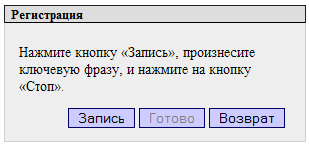
\includegraphics[width=72mm]{static_include/enrollment_created.png}}
\caption{Регистрация: инициализация сессии записи}
\label{fig:enrollment_created}
\end{figure}

При выборе кнопки <<Запись>> начинается запись, и форма  автоматически переходит
в состояние, изображенное на рисунке~\ref{fig:enrollment_recording}. В
центральной части формы отражается состояние времени записи. В нижней части,
заменяя кнопку <<Запись>>, появляется кнопка <<Стоп>>, при нажатии на которую
происходит остановка записи.


\begin{figure}[hbt!]
\center{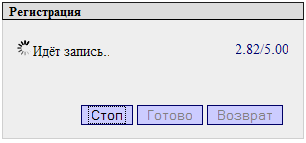
\includegraphics[width=72mm]{static_include/enrollment_recording.png}}
\caption{Регистрация: запись голосового образца}
\label{fig:enrollment_recording}
\end{figure}

Если записанный образец слишком короткий, то при выборе кнопки <<Стоп>>, форма переходит в состояние, представленное на рисунке~\ref{fig:enrollment_too_short_to_upload}. В центре формы находится сообщение о длительности образца и рекомендации пользователю. Из данной формы можно перейти в состояние записи голосового образца или вернуться на главную страницу системы голосовой аутентификации.


\begin{figure}[hbt!]
\center{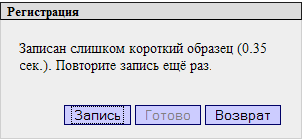
\includegraphics[width=72mm]{static_include/enrollment_too_short_to_upload.png}}
\caption{Регистрация: недостаточно данных для отправления}
\label{fig:enrollment_too_short_to_upload}
\end{figure}

Если образец имеет достаточную длину, форма
(рисунок~\ref{fig:enrollment_recording}) переходит в состояние, представленное
на рисунке~\ref{fig:enrollment_uploading}. В этом состоянии происходит
отправление записи, что отражается в  центральной части формы, также там
отражено время последней записи.


\begin{figure}[hbt!]
\center{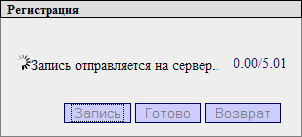
\includegraphics[width=72mm]{static_include/enrollment_uploading.png}}
\caption{Регистрация: отправление записи}
\label{fig:enrollment_uploading}
\end{figure}


При возникновении ошибки во время отправления записи, форма переходит в состояние, представленное на рисунке~\ref{fig:enrollment_upload_error}. В центральной части формы расположено сообщение об ошибке и рекомендации пользователю. 


\begin{figure}[hbt!]
\center{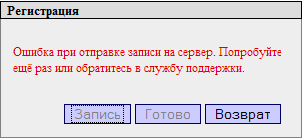
\includegraphics[width=72mm]{static_include/enrollment_upload_error.png}}
\caption{Регистрация: ошибка при отправлении записи}
\label{fig:enrollment_upload_error}
\end{figure}



При удачном завершении отправления записи на сервер, форма
(рисунок~\ref{fig:enrollment_uploading}) переходит в состояние, изображенное на
рисунке~\ref{fig:enrollment_uploaded}. На форме отражается количество, общая
длительность записей, и сообщение о состоянии записи. Если пользователь хочет
отменить процесс регистрации, необходимо выбрать кнопку <<Возврат>>. Если
пользователь хочет продолжить создание голосовой модели, необходимо выбрать
кнопку <<Запись>>. Когда пользователь запишет достаточное количество образцов
ключевой фразы, становиться активной кнопка <<Готово>>.


\begin{figure}[hbt!]
\center{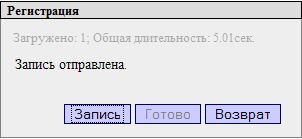
\includegraphics[width=72mm]{static_include/enrollment_uploaded.png}}
\caption{Регистрация: запись отправлена}
\label{fig:enrollment_uploaded}
\end{figure}

При выборе кнопки <<Готово>> начинается процесс обучения модели, и форма переходит в состояние, представленное на рисунке~\ref{fig:enrollment_in_process}. В центральной части формы расположено сообщение о состоянии процесса обучения.

\begin{figure}[hbt!]
\center{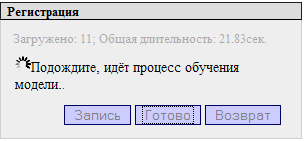
\includegraphics[width=72mm]{static_include/enrollment_in_process.png}}
\caption{Регистрация: обучение модели}
\label{fig:enrollment_in_process}
\end{figure}

Если произошла ошибка при обучении модели, форма переходит в состояние, отраженное на рисунке~\ref{fig:enrollment_error_in_learning}. В центре формы отображается сообщение об ошибке и рекомендации пользователю. При возникновении данной ошибки, пользователь может вернуться на главную страницу системы голосовой аутентификации.

\begin{figure}[hbt!]
\center{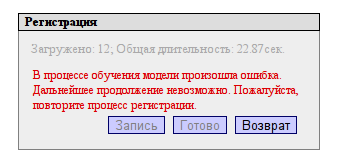
\includegraphics[width=72mm]{static_include/enrollment_error_in_learning.png}}
\caption{Регистрация: ошибка во время обучения модели}
\label{fig:enrollment_error_in_learning}
\end{figure}

Если данных для обучения недостаточно, форма (рисунок~\ref{fig:enrollment_in_process}) переходит в состояние, показанное на рисунке~\ref{fig:enrollment_need_more_data}. В центральной части формы отображается сообщение об ошибке и рекомендации пользователю. При возникновении данной ошибки, пользователь может выбрать кнопку <<Возврат>> или записать дополнительные голосовые данные, выбрав кнопку <<Запись>>.


\begin{figure}[hbt!]
\center{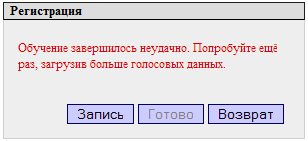
\includegraphics[width=72mm]{static_include/enrollment_need_more_data.png}}
\caption{Регистрация: недостаточно данных для обучения модели}
\label{fig:enrollment_need_more_data}
\end{figure}

При удачном завершении обучения модели, регистрация завершается, и форма (рисунок~\ref{fig:enrollment_in_process}) переходит в состояние, показанное на рисунке~\ref{fig:enrollment_success}. Из этого состояния происходит переход на главную страницу системы голосовой аутентификации, что отражается в сообщении.   


\begin{figure}[hbt!]
\center{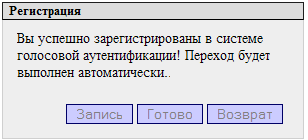
\includegraphics[width=72mm]{static_include/enrollment_success.png}}
\caption{Регистрация: успешное завершение обучения модели}
\label{fig:enrollment_success}
\end{figure}

\subsubsection{Аутентификация по голосу}
\label{sec:manual:verification}


Если на главной странице системы голосовой аутентификации не введено имя учётной записи, то при переходе по  ссылке <<Вход в систему по голосу>>, возникает окно с предупреждением (рисунок~\ref{fig:warning_need_login}). Если имя учётной записи введено, производится переход к странице с формой, которая представлена на рисунке~\ref{fig:verification_created}. Центральная часть формы и функция кнопки <<Запись>> аналогичны описанным в разделе~\ref{sec:manual:enrollment} (рисунок~\ref{fig:enrollment_created}). В нижней части формы находится кнопка <<Возврат>>, при выборе которой, производится переход на главную страницу защищаемого интернет-ресурса.


\begin{figure}[hbt!]
\center{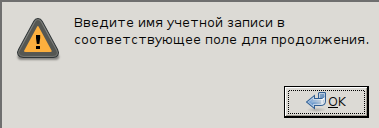
\includegraphics[width=72mm]{static_include/warning_need_login.png}}
\caption{Предупреждение о необходимости ввода имени учётной записи}
\label{fig:warning_need_login}
\end{figure}


\begin{figure}[hbt!]
\center{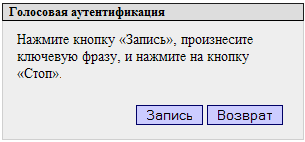
\includegraphics[width=72mm]{static_include/verification_created.png}}
\caption{Аутентификация: инициализация сессии записи}
\label{fig:verification_created}
\end{figure}

Процесс записи ключевой фразы для аутентификации аналогичен процессу записи ключевых фраз для создания индивидуальной голосовой модели. Различие заключается в том, что запись производится один раз, после чего начинается процесс аутентификации (рисунок~\ref{fig:verification_in_process}). 


\begin{figure}[hbt!]
\center{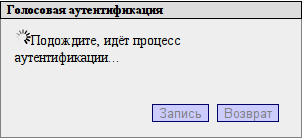
\includegraphics[width=72mm]{static_include/verification_in_process.png}}
\caption{Аутентификация: процесс аутентификации}
\label{fig:verification_in_process}
\end{figure}

Если во время аутентификации произошла ошибка , форма переходит в состояние, отраженное на рисунке~\ref{fig:verification_error}. В центре формы отображается сообщение об ошибке и рекомендации пользователю. При возникновении данной ошибки, пользователь может повторить попытку аутентификации, выбрав кнопку <<Повтор>>, или перейти на главную страницу интернет-ресурса, выбрав кнопку <<Возврат>>. 


\begin{figure}[hbt!]
\center{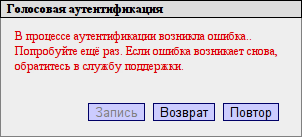
\includegraphics[width=72mm]{static_include/verification_error.png}}
\caption{Аутентификация: ошибка во время аутентификации}
\label{fig:verification_error}
\end{figure}

Если процесс аутентификации завершился отказом в доступе, форма (рисунок~\ref{fig:verification_in_process}) переходит в состояние, показанное на рисунке~\ref{fig:verification_access_denied}. В центре формы отображается сообщение о состоянии аутентификации и рекомендации пользователю. В нижней части формы находятся кнопки <<Возврат>> и <<Повтор>>.


\begin{figure}[hbt!]
\center{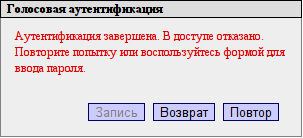
\includegraphics[width=72mm]{static_include/verification_access_denied.png}}
\caption{Аутентификация: в доступе отказано}
\label{fig:verification_access_denied}
\end{figure}

Если аутентификация завершается успешно для пользователя (доступ разрешён), происходит автоматический переход на запрошенную страницу, или на страницу, заданную по-умолчанию, администратором интернет-ресурса.  

\subsubsection{Интерфейс администратора}

На главной странице интерфейса администратора представлен список разделов,
отвечающих за управление соответствующими объектами системы
(рисунок~\ref{fig:admin_main}). Все перечисленные объекты подробно описаны в
разделе~\ref{sec:construct:db}.

\begin{figure}[hbt!]
\center{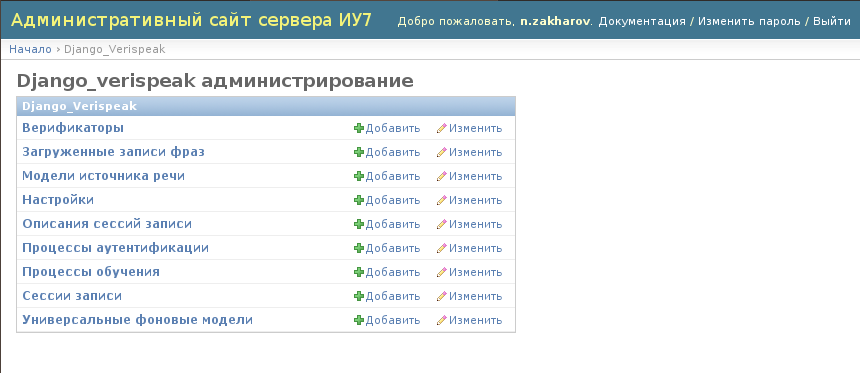
\includegraphics[width=0.8\textwidth]{static_include/admin_main.png}}
\caption{Главное окно интерфейса администратора}
\label{fig:admin_main}
\end{figure}










